\chapter{Methodology}
\label{chapter:prop}

\section{Introduction}

In this chapter, we present an overview of our research methods, highlighting key steps and techniques utilized, with the main objective of developing an accurate and robust \ac{ser} system.

\section{Dataset Collection}

The data collection process involved the selection and acquisition of audio-emotional datasets. The chosen datasets were selected based on their alignment with \ac{sota} research. Preference was given to large and diverse datasets that contained gender-balanced samples and were widely used in the field.

\section{Data Preprocessing}

To enhance the quality of the audio data, a series of preprocessing steps were employed. These included noise reduction techniques to minimize background noise and silence trimming to remove unnecessary portions of the audio signal.

\section{Feature Extraction and Analysis}

The feature extraction process involved extracting relevant audio features from the preprocessed data, such as spectral features, temporal features, and statistical features.

When studying the features extracted from speech audio signals, it is common to consider both global and local features \cite{PORIA201798}. Some emotions are more prominent at the beginning or end of a speech, so it is frequent to consider both global and local features to fully capture the temporal and emotional content of the signal. However, our study focused on global features to simplify the feature representation and streamline the analysis process. Global features provide a holistic representation of the entire audio signal, summarizing its overall characteristics without focusing on specific local segments.

The features were then selected based on their relevance to the \ac{ser} task. Various analysis techniques were applied to the extracted features to gain insights into the underlying patterns and characteristics of the audio data, such as time-domain analysis, frequency-domain analysis, and signal processing algorithms.

\section{Models Implementation}

Two main approaches were employed in model development: a traditional feature-based approach and a deep learning-based approach. The traditional approach involved audio feature engineering, to find a set of suitable audio features, and the selection of appropriate classifiers. The deep learning approach focused on studying the effectiveness of different feature representations and selecting suitable classifiers, which also involved transfer-learning techniques. The models were also then evaluated through cross-dataset validation and compared the results obtained to other \ac{sota} approaches.

\section{Data Stratification}

Data stratification refers to a process of dividing a dataset into subgroups, based on certain properties. We explored different ways of grouping the data and interpreted their effects on the models, this involved stratifying the audio recordings based on various factors, such as duration, speaker genders, and discrete and dimensional annotations. The purpose of data stratification was to address potential biases and improve the performance of the models across different conditions.

\section{\ac{ser} Pipeline}

A versatile and scalable SER pipeline was developed, which involved consuming audio data, detecting voice using a \ac{vad*} tool, and subsequently performing emotion classification on the detected speech segments. The pipeline enabled efficient processing of audio data, in both online and offline time, for performing \ac{ser} tasks.

\ac{vad*} is a technique used in speech processing to identify periods of speech in an audio signal. By focusing on analyzing the voiced speech and ignoring noisy or silent periods, \ac{vad*} can improve the accuracy of a system by reducing the influence of non-speech segments on the analysis. Furthermore, it can decrease the computational cost by reducing the amount of data to be processed. Figure \ref{fig:vad} demonstrates an instance where a \ac{vad*} system is applied to a speech signal, in this case, it is processing chunks with a duration of 1 second. It reduces the original signal of 10 seconds by half by identifying 5 voiced segments that are then fed to a \ac{ser} model \cite{Milling2022}.

\begin{figure}
	\centering
	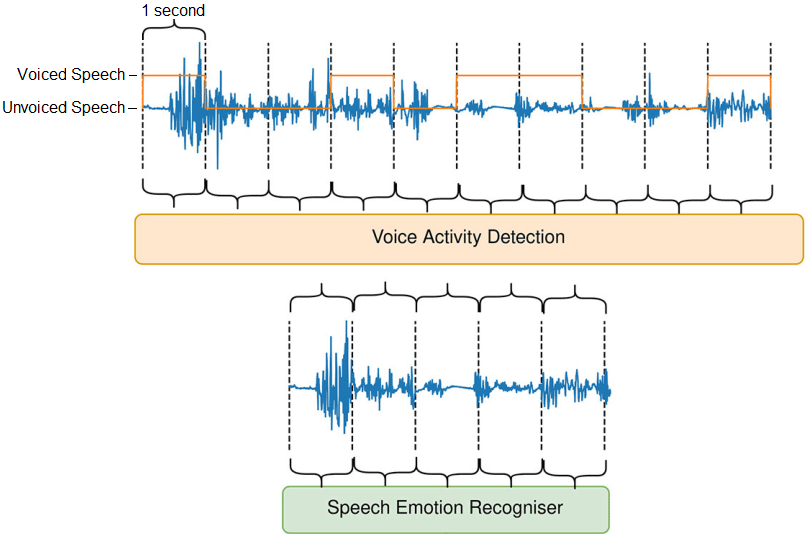
\includegraphics[width=.7\linewidth]{figs/3_methodology/speech_activity_detection.png}
	\caption{\acl{vad*} employment on an audio signal \cite{Milling2022}.}
	\label{fig:vad}
\end{figure}



\section{Ethical Procedures and Concerns}

Ethical considerations were given due attention throughout the research process. The study strictly adhered to ethical guidelines, prioritizing transparency, informed consent, and the protection of personal data.

One ethical concern addressed was the potential bias in the proposed \ac{ser} system's accuracy for individuals with certain characteristics, such as age, gender, accents, or speech disabilities. We conducted an analysis to identify and quantify any biases present in our models, promoting fairness and transparency.

Another ethical concern was the potential misuse of such systems for monitoring or controlling individuals without their consent. Our models are only applied to individuals who have willingly provided their data for emotional evaluation purposes.

To address privacy concerns, our data processing pipelines strictly adhere to principles of data protection. We utilize only the streaming data of participants as input for the \ac{ser} models, and we do not store or use sensitive data for any purposes other than emotional analysis. Additionally, we have chosen not to use speech transcriptions to further safeguard privacy, as they may reveal confidential information.

\section{Conclusion}

The methodology section provided an overview of the research design, data collection, and preprocessing steps, model development approaches, data stratification techniques, the development of the \ac{ser} pipeline, and ethical procedures and concerns. This methodology explains the basis of the subsequent chapters, where the specific details and findings are discussed in more depth.



